See Table \ref{table:2.1.9_sol}.

 \begin{table}[!ht]
	\centering
	\input{./solutions/1-10/table/statexm/statexn92.tex}
	\caption{}
\label{table:2.1.9_sol}
\end{table}
 we can get the mdian by using the ogive graphs.Two types of ogive graphs are used in this method one is less than type ogive and other one is more than type ogive.
\\
 Less than type ogive graph is drawn by using the coordinates of lower limit of class and corresponding comulative frequency.
\\
\begin{figure}[!ht]
	\centering
	\includegraphics[width=\columnwidth]{./solutions/1-10/figures/statexm/statexm9.eps}
	\caption{less than and more than ogives }
	\label{ogive}
\end{figure}
%\begin{lstlisting}
%figure/statexm/statexm9.eps
%\end{lstlisting}
 More than type ogive graph is drawn by using coordinates of upper limit of class and corresponding cumulative frequency.
\\
 the crossing point of the both graph will give 'Median

Related code is available in 
 \begin{lstlisting}
solutions/1-10/codes/statexm/statexm9.py
 \end{lstlisting}
